\documentclass[a4paper,12pt]{article} % добавить leqno в [] для нумерации слева
\usepackage[a4paper,top=1.3cm,bottom=2cm,left=1.5cm,right=1.5cm,marginparwidth=0.75cm]{geometry}
%%% Работа с русским языком
\usepackage{cmap}					% поиск в PDF
\usepackage{mathtext} 				% русские буквы в фомулах
\usepackage[T2A]{fontenc}			% кодировка
\usepackage[utf8]{inputenc}			% кодировка исходного текста
\usepackage[english,russian]{babel}	% локализация и переносы
\usepackage{multirow}

\usepackage{graphicx}

\usepackage{wrapfig}
\usepackage{tabularx}

\usepackage{hyperref}
\usepackage[rgb]{xcolor}
\hypersetup{
colorlinks=true,urlcolor=blue
}

%%% Дополнительная работа с математикой
\usepackage{amsmath,amsfonts,amssymb,amsthm,mathtools} % AMS
\usepackage{icomma} % "Умная" запятая: $0,2$ --- число, $0, 2$ --- перечисление

%% Номера формул
\mathtoolsset{showonlyrefs=true} % Показывать номера только у тех формул, на которые есть \eqref{} в тексте.

%% Шрифты
\usepackage{euscript}	 % Шрифт Евклид
\usepackage{mathrsfs} % Красивый матшрифт

%% Свои команды
\DeclareMathOperator{\sgn}{\mathop{sgn}}

%% Перенос знаков в формулах (по Львовскому)
\newcommand*{\hm}[1]{#1\nobreak\discretionary{}
{\hbox{$\mathsurround=0pt #1$}}{}}

%% Графики
\usepackage{tikz}
\usepackage{pgfplots}
\pgfplotsset{compat=1.9}

\usepackage{subcaption}

\date{\today}

\begin{document}

\begin{titlepage}
	\begin{center}
		{\large МОСКОВСКИЙ ФИЗИКО-ТЕХНИЧЕСКИЙ ИНСТИТУТ (НАЦИОНАЛЬНЫЙ ИССЛЕДОВАТЕЛЬСКИЙ УНИВЕРСИТЕТ)}
	\end{center}
	\begin{center}
		{\large Физтех-школа прикладной математики и информатики}
	\end{center}
	
	
	\vspace{4.5cm}
	{\huge
		\begin{center}
			{\bf Отчёт о выполнении лабораторной работы 3.1.1}\\
			Эффект Хохла
		\end{center}
	}
	\vspace{1cm}
	\begin{center}
		{\large Соболевский Федор Александрович \\
			\vspace{0.2cm}
			Б05-111}
	\end{center}
	\vspace{8cm}
	\begin{center}
		Октябрь 2022
	\end{center}
\end{titlepage}

\section{Аннотация}

В данной работе изучено явление возникновения поперечной ЭДС в полупроводниках с током, находящихся в магнитном поле - эффект Хохла. Исследовано зависимость ЭДС Хохла от величины магнитного поля при различных значениях тока через образец для определения константы Хохла. Также был определён знак носителей заряда и проводимость материала образца.

\section{Теоретические сведения}

\subsection{Эффект Хохла}

\begin{figure}[h]
\centering
    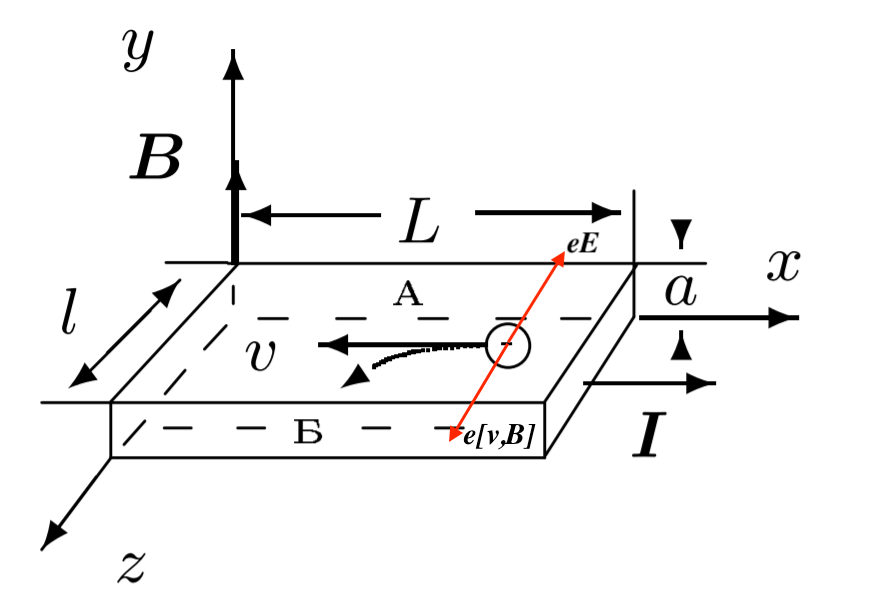
\includegraphics[width=0.7\linewidth]{current.png}
    \caption{Образец с током в магнитном поле}
    \label{fig:current}
\end{figure}

Суть эффекта Хохла состоит в следующем. Пусть через однородную пластину металла вдоль оси $x$ течет ток $I$ (рис.~\ref{fig:current}). Если эту пластину поместить в магнитное поле, направленное по оси y, то между гранями А и Б появляется разность потенциалов. На электрон (для простоты рассматриваем один тип носителей), движущийся со средней скоростью $\langle \vec{v} \rangle$ в электромагнитном поле, действует сила Лоренца:
	
$$\vec{F}_{л} = -e\vec{E}-e \langle \vec{v} \rangle \times \vec{B}$$
	
где $e$~--- абсолютный заряд электрона, $\vec{E}$~--- напряженность электрического поля, $\vec{B}$~--- индукция магнитного поля. В проекции на ось $z$ получаем

$$ F_{B}=e | \langle {v_{x}} \rangle | B.$$
	
Под действием этой силы электроны отклоняются к грани Б, заряжая ее отрицательно. На грани А накапливаются нескомпенсированные положительные заряды. Это приводит к возникновению электрического поля $E_{z}$, направленного от А к Б, которое действует на электроны с силой $F_{E}=eE_{z}$. В установившемся режиме $F_{E}=F_{B}$, поэтому накопление электрических зарядов на боковых гранях пластины прекращается. Отсюда
	
$$ E_{z}=| \langle {v_{x}} \rangle | B.$$
	
С этим полем связана разность потенциалов 

$$U_{AБ}=E_{z}l=| \langle {v_{x}} \rangle | Bl.$$
	
В этом и состоит эффект Хохла. Сила тока в проводнике определяется как
	
$$ I=ne| \langle {v_{x}} \rangle |la.$$
	
Отсюда найдем ЭДС Хохла:
	
\begin{equation}\label{Rx}
	\mathscr{E}_\text{X}=U_\text{AБ}=\dfrac{IB}{nea}=R_\text{X}\dfrac{IB}{a}.
\end{equation}
	
Константа $R_{X}=\dfrac{1}{ne}$ называется постоянной Хохла. В полупроводниках, когда значение проводимости зависит от строения вещества проводника, выражение для постоянной Хохла имеет более сложный вид:
	
$$R_{X}=\dfrac{nb^{2}_{e}-pb^{2}_{p}}{e(nb_{e}+pb_{p})^{2}},$$
	
где $n$ и $p$~--- концентрации электронов и дырок; $b_{e}$, $b_{p}$~--- их подвижности.

\subsection{Экспериментальная устновка}

Схема экспериментальной установки показана на рис.~\ref{fig:setup}.
	
\begin{figure}[h]
\begin{center}
    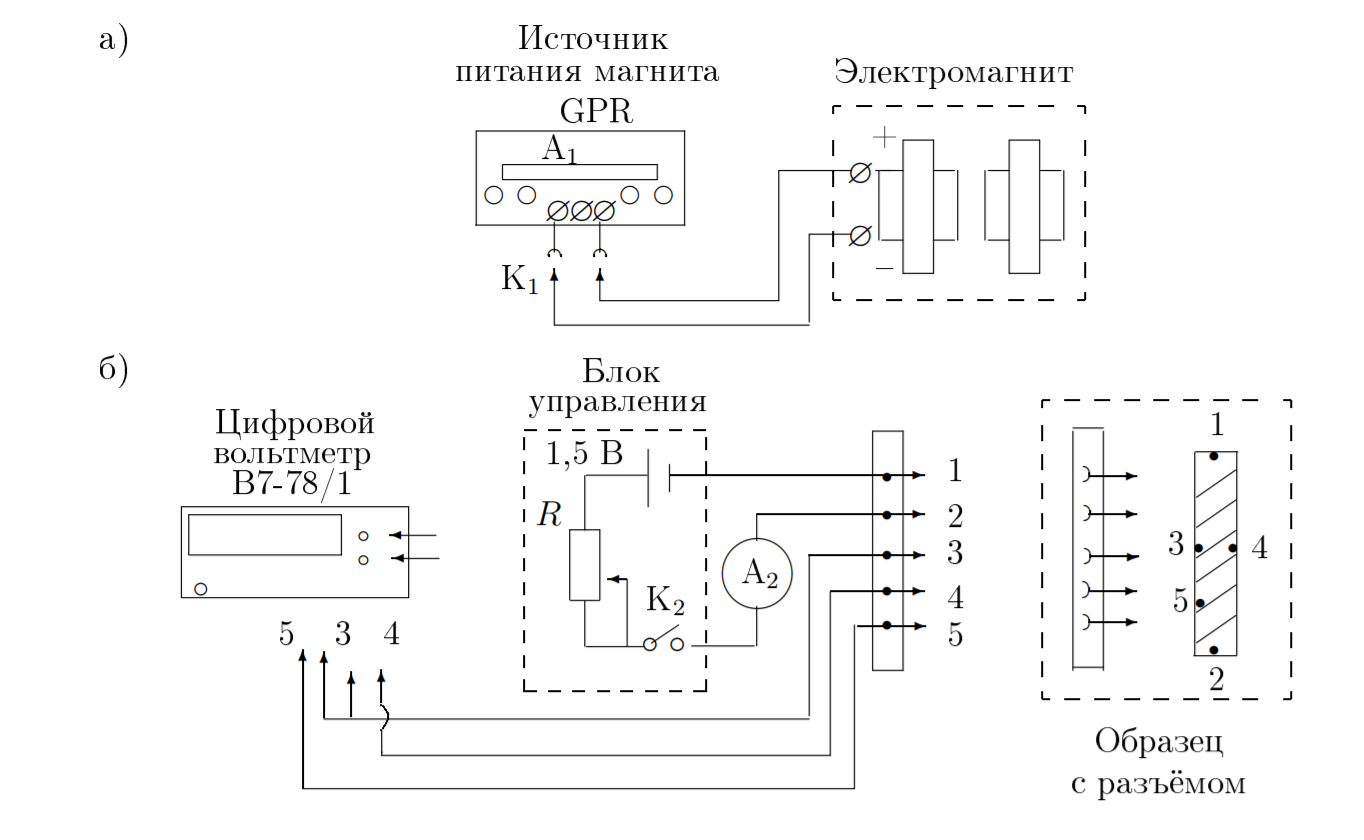
\includegraphics[width=\linewidth]{setup.png}
\end{center}
\caption{Схема установки для исследования эффекта Холла в полупроводниках}
\label{fig:setup}
\end{figure}
  
В зазоре электромагнита (рис.~\ref{fig:setup}a) создаётся постоянное магнитное поле, величину которого можно менять с помощью регуляторов источника питания. Ток измеряется амперметром источника питания $A_{1}$. Разъем $K_{1}$ позволяет менять направление тока в обмотках электромагнита.
  
Образец из легированного германия, смонтированный в специальном держателе (рис.~\ref{fig:setup}б), подключается к батарее. При замыкании ключа $K_{2}$ вдоль длинной стороны образца течет ток, величина которого регулируется реостатом $R$ и измеряется миллиамперметром А$_{2}$.
  	
В образце с током, помещённом в зазор электромагнита, между контактами 3 и 4 возникает разность потенциалов $U_{34}$, которая измеряется с помощью цифрового вольтметра.
  	
Контакты 3 и 4 вследствие неточности подпайки не всегда лежат на одной
эквипотенциали, и тогда напряжение между ними связано не только с эффектом
Хохла, но и с омическим падением напряжения, вызванным протеканием основного тока через образец.
  	
Измеряемая разность потенциалов при одном направлении
магнитного поля равна сумме ЭДС Хохла и омического падения напряжения, а
при другом  их разности. В этом случае ЭДС Хохла $\mathscr{E}_\text{X}$ может быть определена как половина алгебраической разности показаний вольтметра, полученных для
двух противоположных направлений магнитного поля в зазоре.
  	
Можно исключить влияние омического падения напряжения иначе, если при каждом токе через образец измерять напряжение между точками 3 и 4 в отсутствие магнитного поля. При фиксированном токе через образец это дополнительное к ЭДС Холла напряжение $U_{0}$ остается неизменным. От него следует (с учетом
знака) отсчитывать величину ЭДС Хохла: 
  	
$$\mathscr{E}_\text{X} = U_{34} - U_{0}.$$
  	
При таком способе измерения нет необходимости проводить повторные измерения с противоположным направлением магнитного поля.
  	
По знаку $\mathscr{E}_{X}$ можно определить характер проводимости~--- электронный или дырочный. Для этого необходимо знать направление тока в образце и направление
магнитного поля.
  	
Измерив ток $I$ в образце и напряжение $U_{35}$ между контактами 3 и 5 в отсутствие магнитного поля, можно, зная параметры образца, рассчитать проводимость материала образца по формуле:
  	
\begin{equation}\label{sigma}
  \sigma=\dfrac{IL_{35}}{U_{35}ah},
\end{equation}
  	
где $L_{35}$~--- расстояние между контактами 3 и 5, $a$~--- ширина образца, $h$~--- его толщина.
  	
\section{Оборудование и экспериментальные погрешности}

\textbf{Оборудование:} электромагнит с регулируемым источником питания, вольтметр, амперметр, миллиамперметр, миллитесламетр, источник питания, образцы легированного германия.

\textbf{Инструментальные погрешности:}

\begin{itemize}
    \item Амперметр: $\Delta_I = 0,01$ А;
    \item Вольтметр: $\Delta_U = 0,001$ мВ;
    \item Миллиамперметр: $\Delta_\text{мА} = 0,01$ мА;
    \item Миллитесламетр: $\Delta_B = 0,5$ мТл.
\end{itemize}

\section{Результаты измерений и обработка экспериментальных данных}

Параметры образца: $a = 2,2$~мм, $L = 6,0$~мм, $l = 7$~мм. Результаты измерения калибровочной зависимости поля $B$ от тока в электромагните $I_М$ представлены в таб.~\ref{tab1}. В дальнейшем использовались только измеренные значения тока и соответствующие им значения индукции поля. 

\begin{table}[h!]
\begin{center}
\begin{tabular}{|c|c|}
\hline
$I_М$, А & $B$, мТл \\ \hline
0,00 & 22,4 \\ \hline
0,25 & 263,5 \\ \hline
0,50 & 522,6 \\ \hline
0,75 & 762,0 \\ \hline
1,00 & 923,1 \\ \hline
1,25 & 1035,1 \\ \hline
1,50 & 1086,0 \\ \hline
\end{tabular}
\end{center}
\caption{Калибровочная зависимость $B(I_\text{М})$}
\label{tab1}
\end{table}

Результаты измерений разности потенциалов $U_{34}$ между точками 3 и 4 в зависимости от поля $B$ при различных значениях тока через образец $I$ и полученные значения ЭДС Хохла $U_{\perp}$ представлены в таб.~\ref{tab2}-\ref{tab3}. График семейства характеристик $U_{\perp}(B)$ при разных значениях тока $I$ через образец представлен на рис.~\ref{plot1}.

\begin{table}[h!]
\begin{center}
\begin{tabular}{|c|c|c|c|c|}
\hline
$I$, мА & $U_0$, мВ & $I_\text{М}$, А & $U_{34}$, мВ & $U_{\perp}$, мB \\ \hline
\multirow{6}{*}{0,2} & \multirow{6}{*}{$+0,005$} & 0,25 & -0,005 & -0,010 \\ \cline{3-5}
& & 0,50 & -0,013 & -0,018 \\ \cline{3-5}
& & 0,75 & -0,022 & -0,027 \\ \cline{3-5}
& & 1,00 & -0,028 & -0,033 \\ \cline{3-5}
& & 1,25 & -0,032 & -0,037 \\ \cline{3-5}
& & 1,50 & -0,035 & -0,040 \\ \hline
\multirow{6}{*}{0,4} & \multirow{6}{*}{$+0,011$} & 0,25 & -0,006 & -0,017 \\ \cline{3-5}
& & 0,50 & -0,025 & -0,036 \\ \cline{3-5}
& & 0,75 & -0,042 & -0,053 \\ \cline{3-5}
& & 1,00 & -0,054 & -0,065 \\ \cline{3-5}
& & 1,25 & -0,062 & -0,073 \\ \cline{3-5}
& & 1,50 & -0,068 & -0,079 \\ \hline
\multirow{6}{*}{0,6} & \multirow{6}{*}{$+0,018$} & 0,25 & -0,008 & -0,026 \\ \cline{3-5}
& & 0,50 & -0,036 & -0,054 \\ \cline{3-5}
& & 0,75 & -0,060 & -0,076 \\ \cline{3-5}
& & 1,00 & -0,079 & -0,097 \\ \cline{3-5}
& & 1,25 & -0,092 & -0,110 \\ \cline{3-5}
& & 1,50 & -0,100 & -0,118 \\ \hline
\multirow{6}{*}{0,8} & \multirow{6}{*}{$+0,025$} & 0,25 & -0,010 & -0,035 \\ \cline{3-5}
& & 0,50 & -0,046 & -0,071 \\ \cline{3-5}
& & 0,75 & -0,081 & -0,106 \\ \cline{3-5}
& & 1,00 & -0,105 & -0,130 \\ \cline{3-5}
& & 1,25 & -0,121 & -0,146 \\ \cline{3-5}
& & 1,50 & -0,133 & -0,158 \\ \hline
\multirow{6}{*}{1,0} & \multirow{6}{*}{$+0,032$} & 0,25 & -0,013 & -0,045 \\ \cline{3-5}
& & 0,50 & -0,057 & -0,089 \\ \cline{3-5}
& & 0,75 & -0,099 & -0,131 \\ \cline{3-5}
& & 1,00 & -0,132 & -0,164 \\ \cline{3-5}
& & 1,25 & -0,152 & -0,184 \\ \cline{3-5}
& & 1,50 & -0,166 & -0,198 \\ \hline
\end{tabular}
\end{center}
\caption{Результаты измерения ЭДС Хохла при $I = 0,2$\,--\,$1,0$~мА}
\label{tab2}
\end{table}

\begin{table}[h!]
\begin{center}
\begin{tabular}{|c|c|c|c|c|}
\hline
$I$, мА & $U_0$, мВ & $I_\text{М}$, А & $U_{34}$, мВ & $U_{\perp}$, мB \\ \hline
\multirow{6}{*}{1,0} & \multirow{6}{*}{$+0,039$} & 0,25 & 0,084 & 0,045 \\ \cline{3-5}
& & 0,50 & 0,128 & 0,089 \\ \cline{3-5}
& & 0,75 & 0,170 & 0,131 \\ \cline{3-5}
& & 1,00 & 0,202 & 0,163 \\ \cline{3-5}
& & 1,25 & 0,222 & 0,183 \\ \cline{3-5}
& & 1,50 & 0,237 & 0,198 \\ \hline
\end{tabular}
\end{center}
\caption{Результаты измерения ЭДС Хохла при обратном направлении тока}
\label{tab3}
\end{table}

\begin{figure}[h!]
\centering
\resizebox {0.75\textwidth} {!} {
\begin{tikzpicture}
\begin{axis}[ xlabel = {$B$, мТл}, ylabel = {$|U_\perp|$, мВ}, xmin = 0, xmax = 1150, ymin = 0, ymax = 0.21, minor tick num = 5, legend style={legend style={at={(axis cs:1150, 0.21)},anchor=north west}}]
\addplot[color=black, mark=x, only marks] coordinates{
(263.5, 0.010)
(522.6, 0.018)
(762.0, 0.027)
(923.1, 0.033)
(1035.1, 0.037)
(1086.0, 0.04)
};
\addplot[color=blue, mark=o, only marks] coordinates{
(263.5, 0.017)
(522.6, 0.036)
(762.0, 0.053)
(923.1, 0.065)
(1035.1, 0.073)
(1086.0, 0.079)
};
\addplot[color=purple, mark=triangle, only marks] coordinates{
(263.5, 0.026)
(522.6, 0.054)
(762.0, 0.076)
(923.1, 0.097)
(1035.1, 0.11)
(1086.0, 0.118)
};
\addplot[color=black, mark=square, only marks] coordinates{
(263.5, 0.035)
(522.6, 0.071)
(762.0, 0.106)
(923.1, 0.130)
(1035.1, 0.146)
(1086.0, 0.158)
};
\addplot[color=blue, mark=*, only marks] coordinates{
(263.5, 0.045)
(522.6, 0.089)
(762.0, 0.131)
(923.1, 0.164)
(1035.1, 0.184)
(1086.0, 0.198)
};
\legend{$I = 0.2$ мА, $I = 0.4$ мА, $I = 0.6$ мА, $I = 0.8$ мА, $I = 1.0$ мА}
\addplot[color=black, domain=0:1150]{0.000036*x};
\addplot[color=blue, domain=0:1150]{0.000073*x};
\addplot[color=purple, domain=0:1150]{0.000108*x};
\addplot[color=black, domain=0:1150]{0.000144*x};
\addplot[color=blue, domain=0:1150]{0.00018*x};
\end{axis}
\end{tikzpicture}
}
\caption{Графики зависимости ЭДС Хохла в образце от величины магнитного поля и тока}
\label{plot1}
\end{figure}

Знак потенциала соответствует заряду на 3 контакте, значит на нём будут скапливаться дырки. Исходя из геометрии образца, изображённой на рис.~\ref{ris3}, получаем, что основными носителями заряда являются дырки, т. е. имеет место дырочная проводимость.

\begin{figure}[h]
\begin{center}
    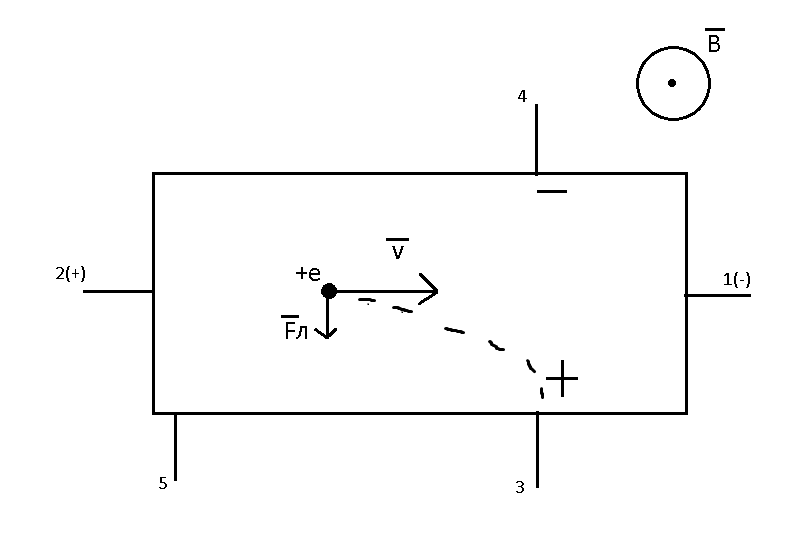
\includegraphics[scale=0.5]{pic.png}
\end{center}
\caption{Направление тока, вектора магнитного поля и отклонение носителей}
\label{ris3}
\end{figure}

График зависимости $k = \frac{|dU_{\perp}|}{dB}$ от тока $I$ представлен на рис.~\ref{plot2}. Получаем угловой коэффициент $\alpha = (18,5\pm0,5)\cdot 10^{-5}~\frac{\text{В}}{\text{А} \cdot \text{Тл}}$. Тогда постоянная Холла $$R_H = \alpha \cdot h = (739\pm35) \cdot 10^{-6}~\frac{\text{м}^3}{\text{Кл}}.$$

\begin{figure}[h!]
\centering
\resizebox {0.55\textwidth} {!} {
\begin{tikzpicture}
\begin{axis}[ xlabel = {$I$, мА}, ylabel = {$k,\,10^{-5}$ В/Тл}, xmin = 0, xmax = 1.1, ymin = 0, ymax = 20, minor tick num = 4]
\addplot[color=black, mark=x, only marks] coordinates{
(0.2, 3.62) 
(0.4, 7.39)
(0.6, 11)
(0.8, 14.7)
(1, 18.5)
};
\addplot[color=blue, domain=0:1.2]{18.5*x};
\end{axis}
\end{tikzpicture}
}
\caption{График зависимости коэффициента пропорциональности $k$ от тока в образце}
\label{plot2}
\end{figure}

Рассчитаем концентрацию носителей заряда по формуле $n = \frac{1}{R_H q} = (8,5\pm0,2) \cdot 10^{21}~\frac{1}{\text{м}^3}$.

При токе $I = 1$~мА разность потенциалов между контактами 3 и 5 \newline $U_{35} = -1,980\pm0,001~\text{В}$. Вычислим удельную проводимость по формуле \eqref{sigma}: \newline $\sigma_0 = 196,7\pm16,1~{\text{Ом} \cdot \text{м}}^{-1}$. Тогда удельное сопротивление $$\rho_0 = 1/\sigma_0 = 0,0050\pm0,0004~{\text{Ом} \cdot \text{м}}.$$

Подвижность носителей заряда рассчитывается по формуле $$\mu = \frac{\sigma}{e n} = 1446\pm123~\frac{\text{см}^2}{\text{В} \cdot \text{с}}.$$

\section{Обсуждение результатов и выводы}

В данной работе были определены постоянная Хохла, подвижность и концентрация носителей заряда в образце легированного германия. Полученные значения:
$$\boxed{R_H = (739\pm35) \cdot 10^{-6}~\frac{\text{м}^3}{\text{Кл}}, \quad n = (8,5\pm0,2) \cdot 10^{21}~\frac{1}{\text{м}^3}, \quad \mu = 1446\pm123~\frac{\text{см}^2}{\text{В} \cdot \text{с}}}$$

Табличное значение собственной концентрации носителей зарядов для германия $n_0 = 2,4~\cdot~10^{22}~\frac{1}{\text{м}^3}$. Это несколько отличается от полученного значения, что говорит о возможном наличии примесей в использованном образце германия. Основной вклад в погрешность вносит погрешность определения коэффициентов зависимости. Также на ошибку измерений может влиять зависимость концентрации основных носителей заряда от температуры, ярко выраженная в полупроводниках.

В ходе работы удалось пронаблюдать эффект Хохла в полупроводнике с током и установить характер проводимости по количественным и качественным характеристикам данного эффекта. Примерное соответствие результатов работы теоретической модели и относительно небольшая погрешность ($<10\%$) говорит о применимости использованного оборудования для наблюдения данного эффекта.

\end{document}